%%%%%%%%%%%%%%%%%%%%%%%%%%%%%%%%%%%%%%%%%%%%%%%%%%%%%%%%%%%%%%%%%%%%%%%%%%%%%%%
% CAPÍTULO 1 – INTRODUÇÃO
%%%%%%%%%%%%%%%%%%%%%%%%%%%%%%%%%%%%%%%%%%%%%%%%%%%%%%%%%%%%%%%%%%%%%%%%%%%%%%%

\chapter{Introdução}
\label{chap:introducao}

O presente trabalho tem como objetivo realizar uma análise aprofundada da experiência do LabTech – a Fábrica de Software Acadêmica do Centro Universitário do Distrito Federal (UDF) – com vistas a identificar gargalos, dificuldades e oportunidades de aprimoramento dos processos internos. Essa análise visa também a proposição de artefatos que reflitam a realidade observada durante a execução dos projetos, dentre os quais destacam-se:

\begin{itemize}[label=\textbullet]
    \item Um edital atualizado, que contemple as práticas reais e a dinâmica operacional do LabTech;
    \item Um modelo padronizado de diário de bordo para os alunos-gerentes, contendo 10 entradas correspondentes às reuniões obrigatórias, que possibilite o registro sistemático das atividades;
    \item Uma lista de tipos de atividades com pontuações associadas, permitindo uma avaliação quantitativa da participação dos alunos, condicionando a obtenção do certificado e/ou estágio obrigatório ao alcance de um número mínimo de pontos.
\end{itemize}

Este trabalho fundamenta-se em relatos de experiência e propostas anteriores, integrando informações de diversos documentos (ver, por exemplo, \cite{rel_danrley_core_2024, rel_labtech_2024_1, rel_labtech_2023_2, rel_lelton_eventos_2024, rel_polyana_2024}). Além disso, amplia a discussão sobre as ferramentas de comunicação, gestão e desenvolvimento utilizadas no ambiente LabTech – como Discord, Trello, Jira, Google Meet, GitHub e Git – e incorpora uma análise quantitativa detalhada com gráficos e figuras que ilustram a dinâmica do projeto.

%%%%%%%%%%%%%%%%%%%%%%%%%%%%%%%%%%%%%%%%%%%%%%%%%%%%%%%%%%%%%%%%%%%%%%%%%%%%%%%
% CAPÍTULO 2 – FUNDAMENTAÇÃO TEÓRICA E REVISÃO DE LITERATURA
%%%%%%%%%%%%%%%%%%%%%%%%%%%%%%%%%%%%%%%%%%%%%%%%%%%%%%%%%%%%%%%%%%%%%%%%%%%%%%%

\chapter{Fundamentação Teórica e Revisão de Literatura}
\label{chap:fundamentacao_literatura}

A evolução das práticas de desenvolvimento de software e a necessidade de integrar teoria e prática no ensino de TI motivaram a criação de Fábricas de Software Acadêmicas. Tais iniciativas, baseadas em conceitos industriais, visam preparar os alunos para os desafios reais do mercado, promovendo a aplicação de metodologias ágeis e a resolução de problemas concretos \cite{dos2021experiencia, neto2017relato}.

\section{Histórico e Conceituação}
O conceito de \textit{Software Factory} foi introduzido pela japonesa Hitachi em 1969 e popularizou-se nos anos 90. Essa abordagem aplica métodos industriais ao desenvolvimento de software, aumentando a produtividade e reduzindo prazos e custos \cite{romanha2016modelo}. No âmbito acadêmico, o LabTech utiliza esse modelo para integrar disciplinas teóricas com a prática de desenvolvimento de soluções que atendam às demandas do meio empresarial, industrial e social.

\section{Importância da Padronização e Coleta de Dados}
A ausência de protocolos padronizados para a coleta de dados – como diários de bordo e relatórios estruturados – dificulta a comparação entre ciclos de desenvolvimento e a mensuração objetiva do desempenho técnico e colaborativo dos alunos \cite{oliveira2017conduccao}. Dessa forma, a definição de \textbf{KPIs} torna-se crucial para:
\begin{itemize}[label=\textbullet]
    \item Monitorar a evolução dos projetos;
    \item Identificar gargalos e áreas de melhoria;
    \item Oferecer feedbacks construtivos para alunos e gestores.
\end{itemize}

\section{Relevância dos Artefatos Propostos}
Diante dos relatos e análises dos documentos \cite{rel_danrley_core_2024, rel_labtech_2024_1, rel_labtech_2023_2}, este trabalho propõe:
\begin{itemize}[label=\textbullet]
    \item A atualização do edital para refletir a prática real do LabTech;
    \item O desenvolvimento de um modelo padronizado de diário de bordo;
    \item A criação de uma tabela de atividades com um sistema de pontuação para avaliação contínua.
\end{itemize}
Esses artefatos visam estabelecer uma cultura de documentação e rastreabilidade, promovendo a transparência e incentivando o desenvolvimento integral dos alunos, tanto do ponto de vista técnico quanto comportamental.

%%%%%%%%%%%%%%%%%%%%%%%%%%%%%%%%%%%%%%%%%%%%%%%%%%%%%%%%%%%%%%%%%%%%%%%%%%%%%%%
% CAPÍTULO 3 – FERRAMENTAS DE COMUNICAÇÃO E GESTÃO
%%%%%%%%%%%%%%%%%%%%%%%%%%%%%%%%%%%%%%%%%%%%%%%%%%%%%%%%%%%%%%%%%%%%%%%%%%%%%%%

\chapter{Ferramentas de Comunicação e Gestão}
\label{chap:ferramentas}

A integração de diversas ferramentas digitais tem sido fundamental para o sucesso do LabTech, permitindo uma comunicação eficiente, o gerenciamento ágil de tarefas e a colaboração em tempo real.

\section{Discord}
O \textbf{Discord} é a principal plataforma de comunicação, onde canais temáticos facilitam discussões técnicas e sociais, além do registro de interações por meio de threads. Esse ambiente colaborativo contribuiu para a transparência das comunicações, conforme indicado nos relatos \cite{rel_danrley_core_2024}.

\section{Trello e Jira}
Para a gestão de tarefas, o LabTech utiliza o \textbf{Trello} e o \textbf{Jira}. O Trello, com sua interface de quadros e cartões, permite uma visualização intuitiva do status das atividades, enquanto o Jira fornece recursos avançados para a gestão de sprints e análise de desempenho, essenciais para o acompanhamento dos projetos em tempo real \cite{rel_labtech_2024_1}.

\section{Google Meet}
O \textbf{Google Meet} é empregado para reuniões virtuais, permitindo o compartilhamento de tela e a gravação das sessões. Essa ferramenta é crucial para o alinhamento das atividades e para a tomada de decisões durante as fases críticas do projeto, conforme evidenciado nos encontros \cite{rel_lelton_eventos_2024}.

\section{GitHub e Git}
O uso do \textbf{GitHub} e do \textbf{Git} para o controle de versão é indispensável. A colaboração é facilitada através de pull requests e revisões de código, embora haja desafios na implementação completa das práticas recomendadas, como o \textit{git flow} e commits convencionais, conforme relatado \cite{rel_danrley_core_2024, rel_labtech_2023_2}.

%%%%%%%%%%%%%%%%%%%%%%%%%%%%%%%%%%%%%%%%%%%%%%%%%%%%%%%%%%%%%%%%%%%%%%%%%%%%%%%
% CAPÍTULO 4 – METODOLOGIA
%%%%%%%%%%%%%%%%%%%%%%%%%%%%%%%%%%%%%%%%%%%%%%%%%%%%%%%%%%%%%%%%%%%%%%%%%%%%%%%

\chapter{Metodologia}
\label{chap:metodologia}

A abordagem metodológica deste trabalho é mista, integrando análises quantitativas e qualitativas para compreender os processos e resultados do LabTech.

\section{Coleta e Análise de Dados}
\subsection{Aspectos Quantitativos}
Os dados quantitativos são extraídos dos repositórios do LabTech e incluem:
\begin{itemize}[label=\textbullet]
    \item Número de \emph{commits}, \emph{issues} e \emph{pull requests};
    \item Frequência e distribuição das contribuições ao longo do tempo;
    \item Métricas de desempenho individual e coletivo, que formam a base para a definição dos \textbf{KPIs}.
\end{itemize}

\subsection{Aspectos Qualitativos}
A análise qualitativa baseia-se na revisão de diários de bordo, relatórios de estágio e registros de reuniões, permitindo identificar desafios de comunicação, dificuldades técnicas e a evolução das competências dos participantes \cite{rel_danrley_core_2024, rel_labtech_2023_2, rel_lelton_eventos_2024, rel_polyana_2024}.

\section{Desenvolvimento dos Artefatos}
Com base na análise dos dados, propõe-se a criação de três artefatos:
\begin{enumerate}[label=\arabic*.]
    \item \textbf{Edital Atualizado:} Revisão do documento atual, incorporando diretrizes que reflitam a prática real e a integração de ferramentas digitais.
    \item \textbf{Modelo de Diário de Bordo:} Um template com 10 entradas obrigatórias, detalhando data, tópicos discutidos, bloqueios, ações e feedbacks.
    \item \textbf{Tabela de Atividades e Sistema de Pontuação:} Uma lista de atividades associadas a valores em pontos, onde o acúmulo mínimo desses pontos valida o estágio e a concessão de certificados.
\end{enumerate}

\section{Integração com Ferramentas e Fluxo de Trabalho}
A comunicação centralizada no Discord, aliada ao uso de threads no GitHub e à gestão de tarefas via Trello/Jira, torna o fluxo de trabalho mais transparente e eficiente, facilitando o acompanhamento das discussões e decisões.

%%%%%%%%%%%%%%%%%%%%%%%%%%%%%%%%%%%%%%%%%%%%%%%%%%%%%%%%%%%%%%%%%%%%%%%%%%%%%%%
% CAPÍTULO 5 – RELATO DE EXPERIÊNCIA
%%%%%%%%%%%%%%%%%%%%%%%%%%%%%%%%%%%%%%%%%%%%%%%%%%%%%%%%%%%%%%%%%%%%%%%%%%%%%%%

\chapter{Relato de Experiência}
\label{chap:relato_experiencia}

Este capítulo consolida os relatos dos ciclos de 2023 e 2024, fornecendo uma visão detalhada dos desafios, aprendizados e feedbacks individuais e coletivos.

\section{Experiência Geral do Projeto}
Durante o ano de 2024, o LabTech passou por diversas fases – da formação inicial da equipe à consolidação dos processos e desenvolvimento de soluções integradas. Conforme o \textit{Relatório Danrley Core 2024} \cite{rel_danrley_core_2024}, o projeto iniciou com um kickoff que visava inspirar os participantes, esclarecendo os objetivos e a natureza do ambiente de aprendizagem. Essa abordagem flexível resultou em variações no nível de comprometimento entre os membros.

\section{Dinâmica de Trabalho e Soft Skills}
Os relatos indicam que as soft skills – como comunicação, trabalho em equipe, autonomia e resiliência – foram determinantes para o sucesso das atividades. Enquanto membros como Guilherme e Nicole demonstraram alta capacidade de aprendizado e colaboração, outros, como Gustavo Saud e Emerson, enfrentaram dificuldades na comunicação e na gestão do tempo, impactando o andamento do projeto. Os diários de bordo ressaltam a importância de registrar não apenas avanços técnicos, mas também desafios emocionais e de comunicação.

\section{Aspectos Técnicos e Desenvolvimento de Soluções}
Os avanços técnicos foram evidentes em diversas áreas:
\begin{itemize}[label=\textbullet]
    \item \textbf{Back-end:} A implementação de uma API robusta em Python (Flask), com autenticação via token, organização em camadas e testes unitários, destacou a importância do acompanhamento dos mentores \cite{rel_danrley_core_2024, rel_labtech_2024_1}.
    \item \textbf{Front-end:} O desenvolvimento em React, embora desafiador na integração com a API e na gestão de estados, evoluiu com contribuições significativas de Nicole \cite{rel_labtech_2023_2}.
    \item \textbf{Integração:} A prática de versionamento com Git, por meio de pull requests e revisões de código, foi fundamental para manter a qualidade do código, embora o domínio completo do \textit{git flow} ainda necessite aprimoramento.
\end{itemize}

\section{Relatos de Encontros e Feedbacks}
Encontros presenciais e virtuais – conforme documentado no \textit{Relatório de Eventos} \cite{rel_lelton_eventos_2024} e no \textit{Relatório da Equipe Polyana} \cite{rel_polyana_2024} – detalharam as discussões sobre a integração das camadas de Controller, Service e Repository, e destacaram a necessidade de aprofundar conhecimentos em conceitos como requisições HTTP, algoritmos e versionamento de código.

%%%%%%%%%%%%%%%%%%%%%%%%%%%%%%%%%%%%%%%%%%%%%%%%%%%%%%%%%%%%%%%%%%%%%%%%%%%%%%%
% CAPÍTULO 6 – RESULTADOS E DISCUSSÃO
%%%%%%%%%%%%%%%%%%%%%%%%%%%%%%%%%%%%%%%%%%%%%%%%%%%%%%%%%%%%%%%%%%%%%%%%%%%%%%%

\chapter{Resultados e Discussão}
\label{sec:discussao-resultados}

A análise dos dados dos repositórios, em conjunto com os relatos dos diários de bordo, possibilitou uma compreensão aprofundada da dinâmica do LabTech.

\section{Aspectos Técnicos}
Os registros indicam que a adoção de frameworks modernos (Spring Boot, Flask, React) contribuiu significativamente para o desenvolvimento das funcionalidades. A implementação de testes unitários e a organização do código em camadas demonstraram a evolução das \emph{hard skills} dos alunos. Contudo, desafios persistem na configuração dos ambientes e na prática de versionamento com Git.

\section{Aspectos Gerenciais}
A ausência de papéis formais (por exemplo, Scrum Master ou Product Owner) e a falta de relatórios padronizados dificultaram a identificação precoce dos gargalos. Reuniões semanais e revisões de código auxiliaram na mitigação de alguns problemas, mas evidenciam a necessidade de protocolos mais rigorosos para a gestão do backlog e a comunicação dos bloqueios.

\section{Aspectos Educacionais}
A experiência demonstrou a importância de desenvolver tanto as \emph{hard skills} quanto as \emph{soft skills}. Embora alguns alunos tenham evoluído significativamente, a variabilidade no desempenho reforça a necessidade de intervenções pedagógicas direcionadas, que permitam uma avaliação longitudinal mais precisa.

\section{Análises Quantitativas}
A seguir, são apresentados gráficos que ilustram a dinâmica do LabTech:

\subsection{Heatmap de Atividade}
\begin{figure}[!htbp]
    \centering
    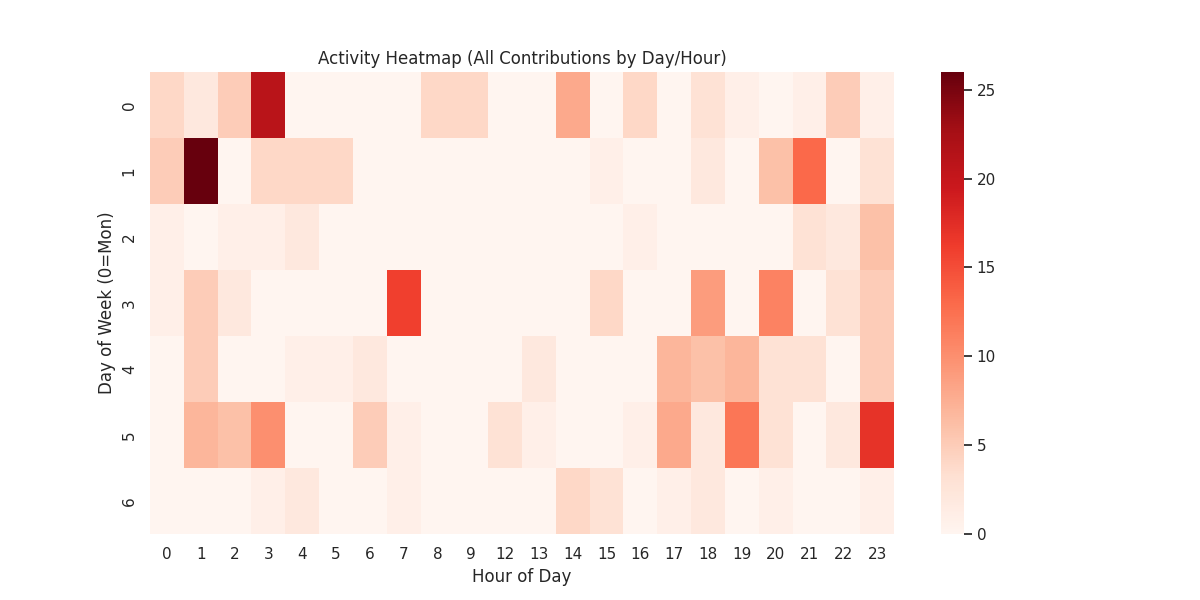
\includegraphics[width=0.7\textwidth]{04-figuras/graficos/github/activity-heatmap.png}
    \caption{Heatmap – Contribuições (commits, issues, pull requests) por Dia e Hora.}
    \label{fig:heatmap_activity}
\end{figure}
O heatmap evidencia a concentração de atividades em horários noturnos e no início da semana, possivelmente devido às rotinas acadêmicas dos participantes.

\subsection{Burndown Chart}
\begin{figure}[!htbp]
    \centering
    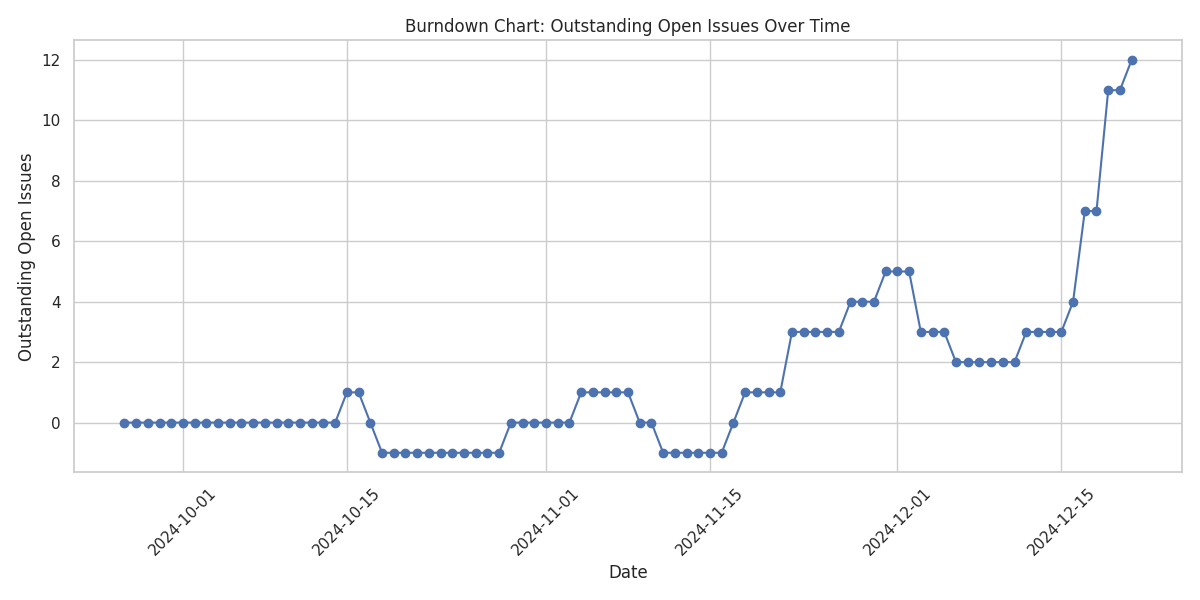
\includegraphics[width=0.7\textwidth]{04-figuras/graficos/github/burndown-chart.png}
    \caption{Burndown Chart – Evolução das \emph{issues} abertas e fechadas.}
    \label{fig:burndown_chart}
\end{figure}
O gráfico mostra períodos de alta e baixa demanda, evidenciando os ciclos de sprint e entregas.

\subsection{Rede de Colaboração}
\begin{figure}[!htbp]
    \centering
    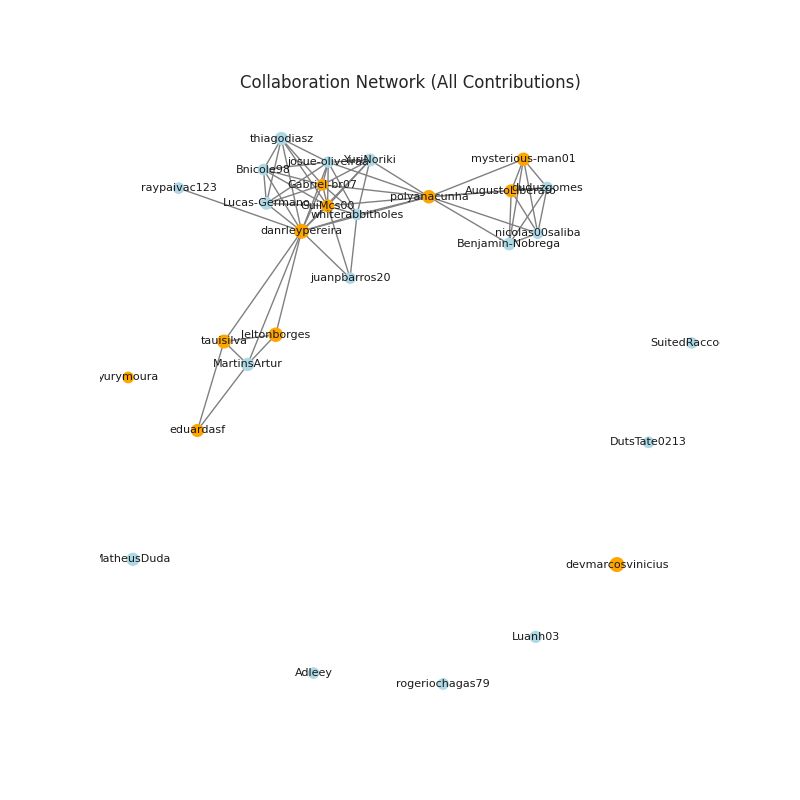
\includegraphics[width=0.65\textwidth]{04-figuras/graficos/github/collaboration-network.png}
    \caption{Rede de Colaboração – Todas as Contribuições.}
    \label{fig:network_all_contribs}
\end{figure}
\begin{figure}[!htbp]
    \centering
    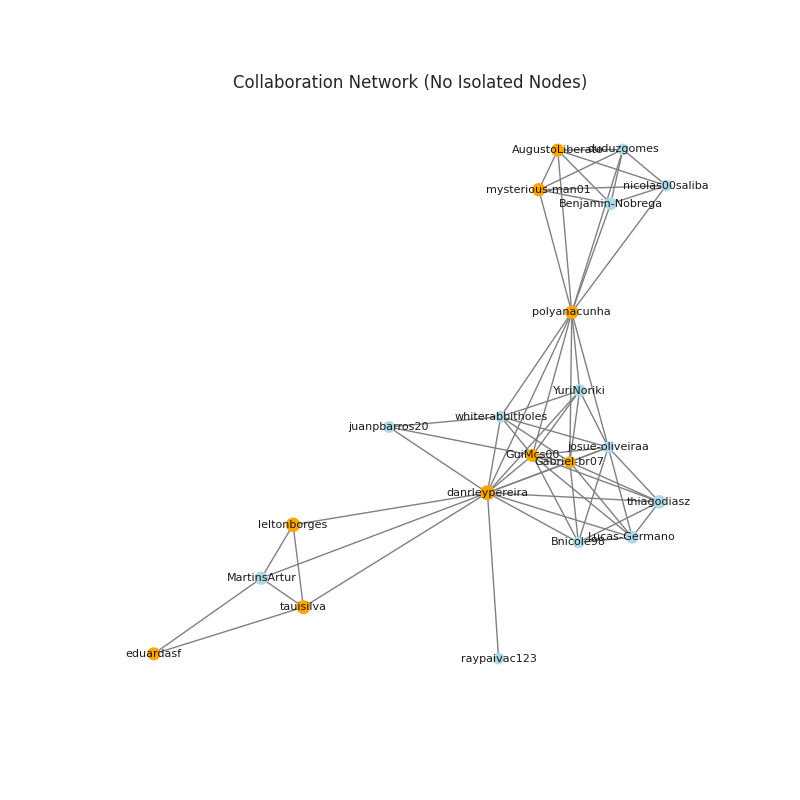
\includegraphics[width=0.65\textwidth]{04-figuras/graficos/github/collaboration-network-no-isolated.png}
    \caption{Rede de Colaboração – Excluindo Nós Isolados.}
    \label{fig:network_no_isolated}
\end{figure}
Essas visualizações ressaltam a importância de integrar os participantes para formar um núcleo colaborativo robusto.

\subsection{Distribuição de Commits}
\begin{figure}[!htbp]
    \centering
    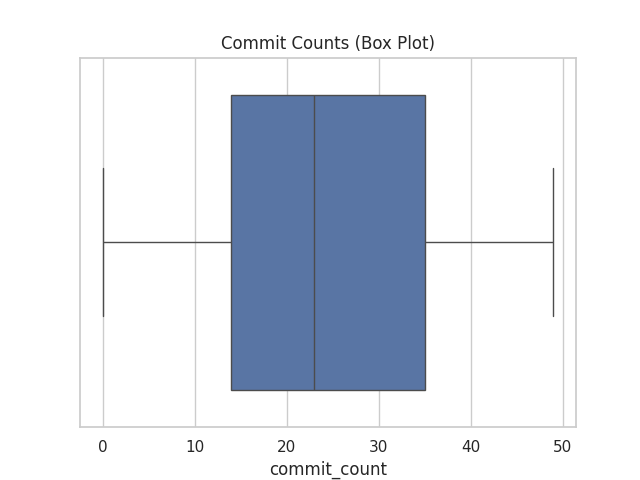
\includegraphics[width=0.55\textwidth]{04-figuras/graficos/github/commit-boxplot.png}
    \caption{Box Plot – Distribuição dos Commits por Membro.}
    \label{fig:commit_boxplot}
\end{figure}
\begin{figure}[!htbp]
    \centering
    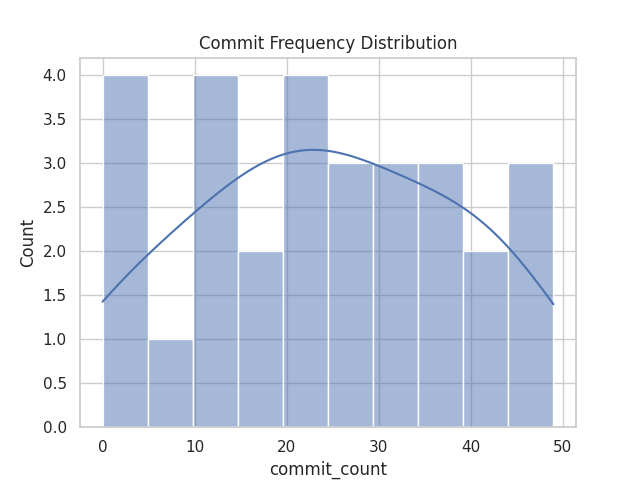
\includegraphics[width=0.6\textwidth]{04-figuras/graficos/github/commit-frequency.png}
    \caption{Histograma – Frequência dos Commits.}
    \label{fig:commit_histogram}
\end{figure}
Esses gráficos indicam disparidades nas contribuições individuais, sugerindo a necessidade de equilibrar a participação.

\subsection{Evolução das Contribuições}
\begin{figure}[!htbp]
    \centering
    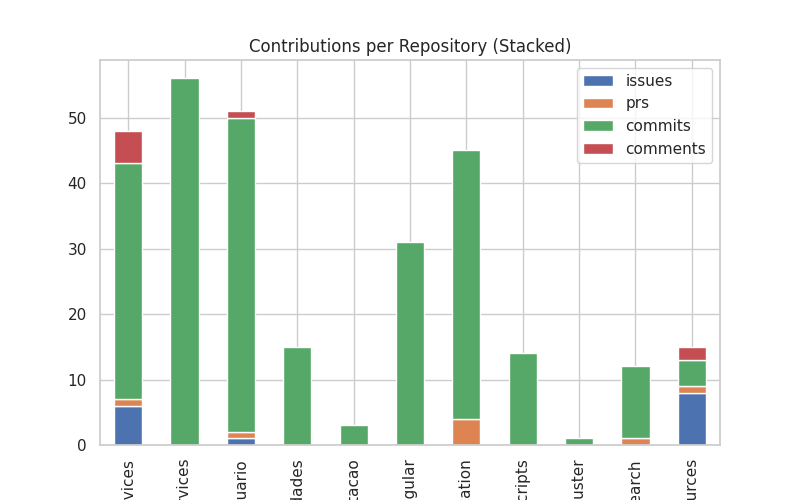
\includegraphics[width=0.75\textwidth]{04-figuras/graficos/github/contributions-per-repo.png}
    \caption{Contribuições por Repositório ao Longo do Tempo.}
    \label{fig:contrib_time_all}
\end{figure}
\begin{figure}[!htbp]
    \centering
    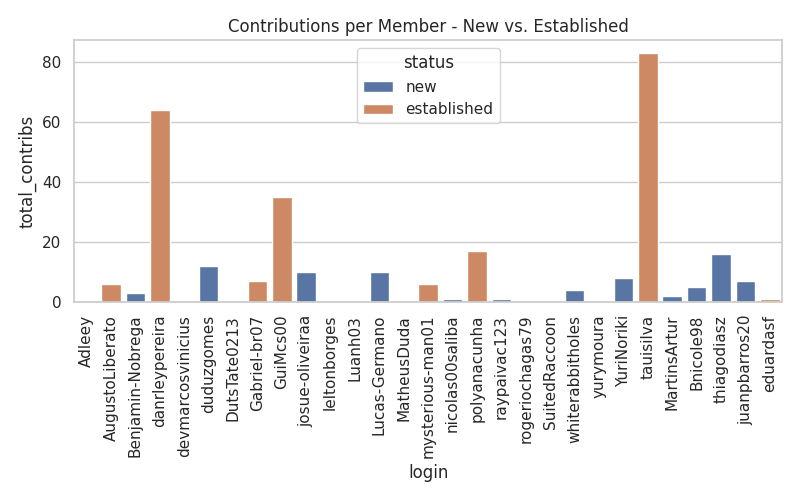
\includegraphics[width=0.75\textwidth]{04-figuras/graficos/github/contributions-per-member.png}
    \caption{Contribuições por Membro (Agosto a Dezembro de 2024).}
    \label{fig:contrib_time_augdec}
\end{figure}
Essas análises quantitativas reforçam a necessidade de estratégias para melhorar a distribuição de tarefas e a comunicação interna.

%%%%%%%%%%%%%%%%%%%%%%%%%%%%%%%%%%%%%%%%%%%%%%%%%%%%%%%%%%%%%%%%%%%%%%%%%%%%%%%
% CAPÍTULO 7 – CONCLUSÕES E TRABALHOS FUTUROS
%%%%%%%%%%%%%%%%%%%%%%%%%%%%%%%%%%%%%%%%%%%%%%%%%%%%%%%%%%%%%%%%%%%%%%%%%%%%%%%

\chapter{Conclusões}
\label{chap:conclusoes}

\section{Considerações Finais}
A análise abrangente da experiência no LabTech evidenciou ganhos significativos nas competências técnicas e interpessoais dos alunos, aproximando a formação acadêmica das exigências do mercado de TI. Apesar dos desafios, como a falta de padronização dos diários de bordo e as dificuldades de comunicação interna, o ambiente tem se mostrado um espaço promissor para a aplicação prática de metodologias ágeis e o desenvolvimento de soluções inovadoras.

A variabilidade no desempenho dos participantes destaca a necessidade de protocolos rigorosos de documentação e de treinamento contínuo para aprimorar tanto as \emph{hard skills} quanto as \emph{soft skills}. Os artefatos propostos – edital atualizado, modelo de diário de bordo e tabela de atividades – serão fundamentais para aprimorar os processos internos e garantir a evolução dos projetos.
